
\begin{figure}[h]  
    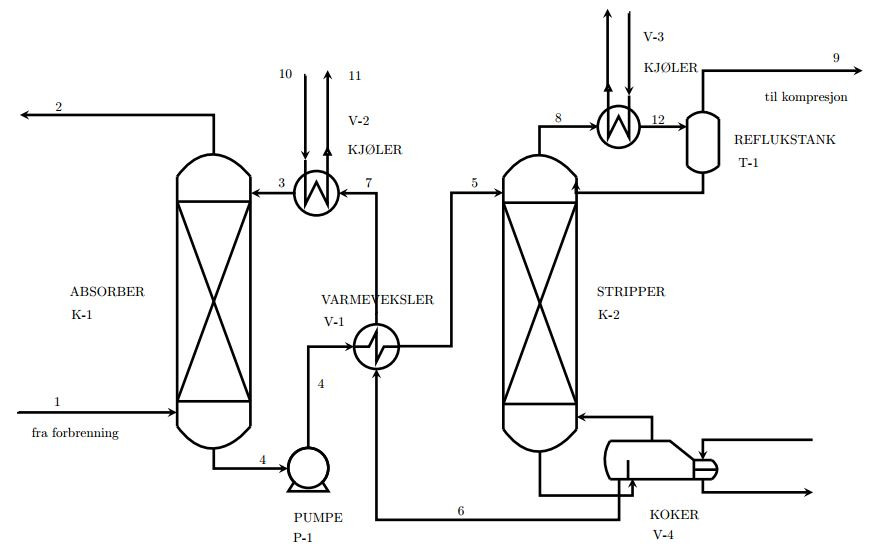
\includegraphics[scale=0.8]{Tegning.JPG}
\centering
\caption{Flytskjema av post-combustion CO\textsubscript{2}-fangst}
\end{figure}

I strøm 1 går røyk av CO\textsubscript{2} og inerte gasser inn, CO\textsubscript{2} blir løst og absorbert av MEA i absorberen. MEA-løsningen går videre i strøm 4 og blir så pumpet gjennom en varmeveksler som varmer opp løsningen, mens CO\textsubscript{2} og inerte gasser går ut gjennom strøm 2. MEA-løsninger går deretter inn i en stripper hvor CO\textsubscript{2} blir spaltet fra MEA. Vann og CO\textsubscript{2} går ut som gass i strøm 8, mens MEA går gjennom kokeren for å sørge for at mer CO\textsubscript{2} blir frigitt. Strøm 8 går gjennom en kjøler slik H\textsubscript{2}O kondensere og CO\textsubscript{2} er fortsatt i gassform. Reflukstanken vil skille disse to og all CO\textsubscript{2} vil gå ut gjennom strøm 9 som eneste komponent, mens vannet vil bli resirkulert inn i stripperen. I strøm 6 vil MEA gå gjennom varmeveksleren for å så bli ytterligere kjølt ned av en kjøler. Dermed blir MEAs kretsløp fulført gjennom strøm 3 som fører tilbake til absorberen. 


I absorberen hvor CO\textsubscript{2} blir absorbert av MEA-løsningen vil det instilles to likevekter. Den ene mellom CO\textsubscript{2}(g) og CO\textsubscript{2}(aq) og den andre mellom CO\textsubscript{2}(aq) og MEA(aq). Vi antar at all CO\textsubscript{2}(aq) blir absorbert av MEA-løsningen. Ved lavere tempraturer blir mer CO\textsubscript{2} absorbert i MEA løsningen.

I stripperen vil MEA-løsningen varmes opp for å frigi mest mulig CO\textsubscript{2}. Her vil løsningen varmet opp for å forskyve likevekten slik at det er mer CO\textsubscript{2} i væskefase og slik at CO\textsubscript{2} og H\textsubscript{2}O vil fordampe over i gassfase.

Varmeveksler V-1 vil varmeveklse strøm 4 mot strøm 6 for å varme opp strøm 4 som skal inn i stripperen og kjøle ned strøm 6 som skal kjøles ned. I kokeren V-4 vil MEA-Løsningen bli varmet opp for å frigi mer CO\textsubscript{2}. Kjøler V-3 vil kjøle ned strøm 8 for å kondensere H\textsubscript{2}O. Kjøler V-2 vil kjøle ned strøm 7 ytterligere slik at strømmen kan ta opp mer CO\textsubscript{2} i absorberen.


\subsection{Reaksjoner}
\import{Oppgaver/}{Reaksjoner.tex}

\subsection{Viktige faktorer i prosessen}
En av de viktigste faktorene for denne prosessen, når det gjelder fanging av CO\textsubscript{2}, vil være MEAs evne til å absorbere CO\textsubscript{2}. Denne faktoren kan deles inn i to deler. Hvor mye CO\textsubscript{2} som kan absorberes av MEA, og hvor raskt MEA absorberer CO\textsubscript{2}. Dette er fordi at selv om det finnes aminer som, i terorien, vil kunne absorbere mer CO\textsubscript{2}, så vil det ikke si at de kan gjøre det i praksis, når vi tar hensyn til tiden det tar å absorbere CO\textsubscript{2}. Et amin som kan absorbere mer CO\textsubscript{2} enn MEA totalt sett, men gjør det over lengere tid enn MEA, vil ikke kunne bruke sitt fulle potensiale når den ikke har tid nok til å absorbere CO\textsubscript{2}en. 

En annen faktor vil være temperaturen på strømmene. En kaldere strøm vil kunne absorbere mer CO\textsubscript{2} (i absorberen) mens en varmere strøm vil kunne gi fra seg mer CO\textsubscript{2} (i strippereren). Det som bestemmer disse egenskapene er varmevekslerens (V-1) effekt, kjølerens (V-2) evne til å kjøle ned strømmen og kokerens (V-4) evne til å varme strømmen, og hvor mye energi som kreves til disse prossesene. 

\subsection{Utfordringer ved prosessen}
I denne rapporten er det lagt hovedvekt på to delprosesser som medfører utfordringer ved hele prosessen.Den første utfordringen er å få absorbert nok CO\textsubscript{2} i absorberen. Det beste hadde vært om man kunne fått absorbert all CO\textsubscript{2} slik at det ikke går CO\textsubscript{2} i gassform ut gjennom strøm 2. Den andre utfordringen er i stripperen der problemet er å spalte CO\textsubscript{2} fra MEA på en mest mulig effektiv måte. Det optimale hadde vært å skille CO\textsubscript{2} fullstendig fra MEA-løsningen, men i realiteten er ikke dette mulig. 

Disse to til sammen medfører stort energibehov for totalprosessen. Dette fordi man må varme opp og kjøle ned strømmene slik at både stripperen og absorberen blir effektiv nok. 

I tillegg har vi utfordinger som at MEA kan deformeres? og må da, etterhvert, byttes ut. Andre utfordinger er at MEA kan fordampe og gå ut i naturen i strøm 2. 
